\newpage

\section{基于数据库系统的数据分析模块实现}

MIDIS平台在设计中,一直很注重对数据的管理。数据库是一种有组织的数据集合,能够提供数据存储,查询,备份的数据管理工具。设计一个高效强大的数据库系统对于MIDIS平台的数据管理和数据安全来说有较大意义。借助数据库系统可以很方便地实现其他数据处理的相关功能。本章将介绍MIDIS数据库系统的设计和基于数据库系统的数据处理模块的实现。

\subsection{数据库设计}

课题组搭建的机群主要是为了给实验室提供仿真计算使用,机群中的计算机可以相互访问。因此,设计一个能够提供相互访问的数据库系统,会数据处理带来极大方便。Python自带的sqlite3[42]是一个轻量级的,不提供ip访问的数据库框架。Mysql是能够提供网络访问的关系型数据库,但是Mysql[43]的语法较为复杂,提供的数据导出功能也并不友好。新出现的非关系型数据库Mongodb[44]能够满足本次设计的要求。Mongodb的特色如表3-1所示。
\begin{figure}[htbp]
	% caption放上面就会显示在图的上方,出现在下面就是出现在图的下方
	% label的位置也有讲究
	\begin{center}
		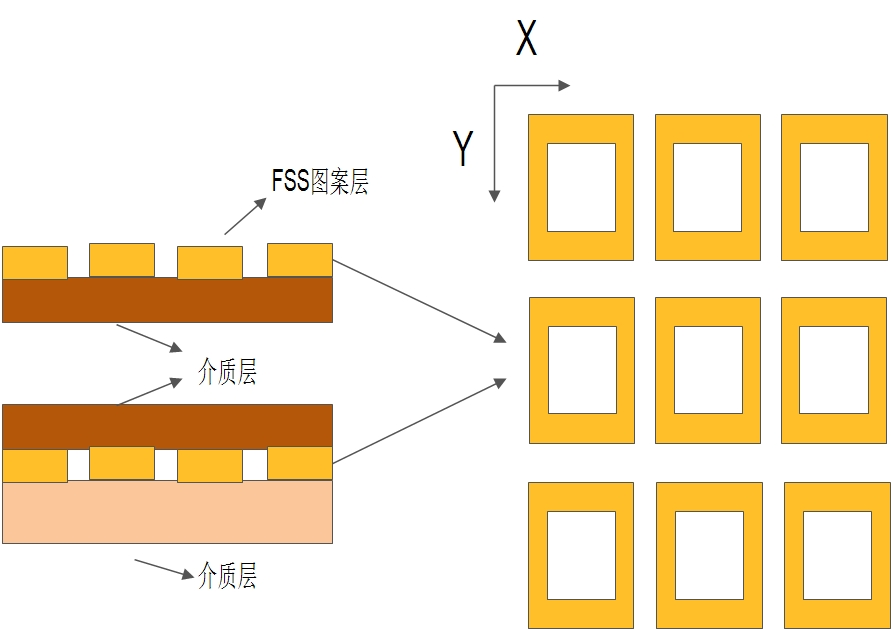
\includegraphics[width=1.0\textwidth]{fssstructure}
		\caption{FSS结构}
		\label{gra4}
	\end{center}
\end{figure}

\begin{equation}
    Recall_u = \frac{|\mathcal{I}_u^{re} \cap \mathcal{I}_u^{te}|}{|\mathcal{I}_u^{te}|}
    \end{equation}